\chapter{Domain Statistics}
To get an overview over the domain and to help make decisions about future evaluations we looked at the domain overall.
We first define concepts used, explain metrics for the evaluations used, look into the domain of Schafkopf followed by
some interesting findings.
\section{Key Concepts}
In order to have clear references in the following sections, we will define and discuss the concepts, methods and
metrics that will help to understand the experiments conducted.

\subsection{Evaluating Player Strength}
The goal of this work is to evaluate an agents playing strength for Schafkopf.
We will outline three main strategies for this, that are reward earned overall, win percentage and expected value.
\subsubsection{Rewards Overall}
After each hand players are awarded a reward (See \ref{scoringphase}).
The total reward earned can be plotted on as Cumulative Sum for all players.
The Cumulative sum after N hands is calculated with:
\newline
\begin{center}
    Let r\textsubscript{i} be the reward earned in hand i then
\begin{equation}
    \text{Reward after N Hands} = \sum_{i=1}^{N} r_{i}
\end{equation}
\newline
\begin{figure}[h]
    \centering
    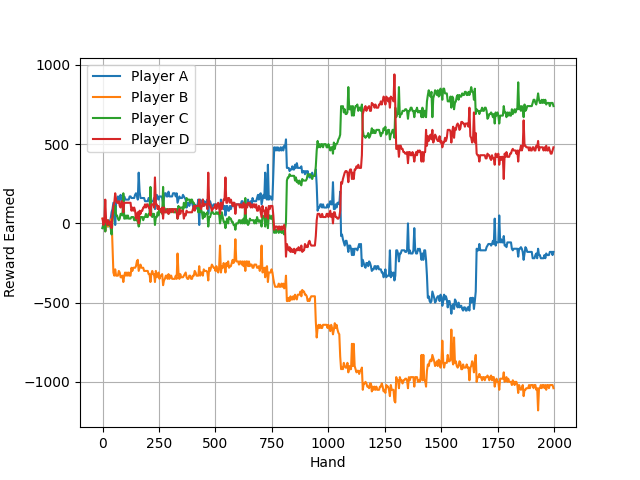
\includegraphics[size=0.75]{expampleRewardEarned.png}
    \caption{Example of Rewards Earned for 4 Players after 2000 hands}
    \label{fig:exampleCumSum}
\end{figure}
\end{center}
See Figure \ref{fig:exampleCumSum} for an example of this.\newline
This metric can be useful to get an initial idea of who is winning, but is susceptible to variance.\newline
Repeated trials often produce different results for players of equal strength.
\subsubsection{Win Percentage}
Firstly one can look at the overall win percentages across a sample of hands.
The win percentage can be calculated with the following formula.
\[\text{Win \%} = \frac{\# \text{ Hands Won}}{\# \text{ Hands Played}}\]
TODO example table
To achieve more detail of the agent's performance one we can further split the win percentage up into roles.
Overall there are seven roles in Schafkopf depending on the game mode, four offensive and three opposition:
\begin{itemize}
    \item Team
    \item Wenz
    \item Solo
    \item Team-Partner
    \item Team-Opposition
    \item Wenz-Opposition
    \item Solo-Opposition
\end{itemize}
For each of the seven roles we can then calculate separate win percentages with the formula above, replacing the
\textbf{Hands Won} and \textbf{Hands Played} with the respectively subset for each role.
\newline
This results for each player can then be shown in a table that allows for easy analysis of each role.
\newline
\begin{table}
\begin{tabular}{lrrrrrrr}
    \toprule
    Player & Team & Wenz & Solo & Team-Partner & Team-Opp & Wenz-Opp & Solo-
    Opp \\
    \midrule
    PlayerA & 0.506 & 0.917 & 0.864 & 0.527 & 0.505 & 0.167 & 0.226 \\
    PlayerB & 0.474 & 0.875 & 0.729 & 0.509 & 0.480 & 0.153 & 0.181 \\
    PlayerC & 0.527 & 1.000 & 0.829 & 0.518 & 0.511 & 0.194 & 0.214 \\
    PlayerD & 0.516 & 0.625 & 0.764 & 0.470 & 0.481 & 0.069 & 0.193 \\
    \bottomrule
\end{tabular}
\caption{Example of \textbf{winning percentage} for all seven roles for four players}
\label{winpercentageroles}
\end{table}
\newline
Win percentages are useful and would be sufficient if it were not for extra rewards \textit{Schneider} and
\textit{Schwarz}.
Two agents may have the same \textbf{winning percentage}, but one agent accumulates more rewards.

\subsubsection{Expected Value}
To address this we use \textbf{Expected Value(EV)}.
This concept is common in gambling games to express how much a certain bet or action, in our case hand, returns over
a large sample.
The formula used is the arithmetic mean:
\[ \text{EV} = \frac{1}{n} \sum_{i=1}^{n}a_{i} = \frac{a_{1} + a_{2} + ...+a_{n}}{n} \]
There are two hand metrics we can use for \textit{a\textsubscript{i}} of achieving this: \textbf{Points Scored} and
\textbf{Reward Earned}.
\subsubsection{Points Scored}
To calculate \textbf{EV\textsubscript{Points Scored}} of the hand sample we record the points scored and use the
above \textbf{EV} formula to calculate the metric.
\newline
\begin{table}[!h]
\centering
\begin{tabular}{cccc}
\toprule
Player A &  Player B &  Player C &  Player D\\
\midrule
32.48 & 33.71 & 27.49 & 26.32 \\
\bottomrule
\end{tabular}
\caption{EV\textsubscript{Points Scored} after 10000 games for four Players}
\label{tab:evscorestable}
\end{table}
\newline
In Table \ref{tab:evscorestable} we can see that Player A can expect to score 32.48 points per hand compared to only
the 26.32 of Player D.
In general we can say that Player A is the better player compared to Player B.
\newline
Although \textbf{EV\textsubscript{Points Scored}}certainly tells us something about playing strength, since Schafkopf
is after all a trick game, it also does not tell the whole story.
This metric scores greedy agents that only score for themselves higher than an agent that plays cooperative, even
though the cooperative agent might win more \textbf{Rewards} or even have a higher \textbf{Winning Percentage}.
\newline
It may certainly be useful but is not suitable to clearly evaluate an agent's playing strength.
Additionally one might also split up \textbf{EV\textsubscript{Points Scored}} further into the seven game role
categories, but this approach seems equally flawed.

\subsubsection{Rewards Earned}
To calculate \textbf{EV\textsubscript{Rewards Earned}} of the hand sample we record the rewards earned and use the
above \textbf{EV} formula to calculate the metric.
\newline
\begin{center}
\begin{table}[h!]
\begin{tabular}{cccc}
\toprule
Player A &  Player B &  Player C &  Player D\\
\midrule
2.32 &              2.92 &          -2.15 &          -3.08 \\
\bottomrule
\end{tabular}
\caption{Example of EV\textsubscript{Rewards Earned} after 10000 games for four Players}
\label{tab:EVrewardsOverall}
\end{table}
\end{center}
Table \ref{tab:EVrewardsOverall}] shows for example that Player A can expect +2.32 \textit{Reward} per hand, while
Player D can expect to lose -3.08 \textit{Reward} per hand.
To look closer at the areas that cause this we can also look again at the game roles.
\newline
\begin{center}
\begin{table}[h!]
\begin{tabular}{lrrrrrrr}
\toprule
Player &  Team &    Wenz &   Solo &  Team-Partner &  Sauspiel-Opp &  Wenz-Opp &  Solo-Opp \\
\midrule
Player A &  4.93 &   39.58 &  84.39 &          2.39 &         -0.48 &     87.89 &     -2.83 \\
Player B &  4.27 &  131.48 &  79.03 &          6.08 &          1.61 &    -47.73 &     -6.85 \\
Player C &  2.03 &  -21.07 &  13.42 &         -2.21 &         -5.46 &    -34.35 &    -80.14 \\
Player D & -2.88 &  -23.68 &   6.31 &          1.51 &         -6.18 &   -235.00 &    -98.13 \\
\bottomrule
\end{tabular}
    \caption{Example of EV\textsubscript{Rewards Earned} by game role after 10000 games for four Players}
\label{tab:EVrewardsGamemode}
\end{table}
\end{center}
\textbf{EV\textsubscript{Rewards Earned}} overcomes the previous pitfall.
It more accurately shows when agents extract value from additional rewards earned, which was not possible by simply
looking at the \textbf{Winning Percentages}, or while also taking into account the advantage of cooperative play.
\newline
\textbf{EV\textsubscript{Rewards Earned}} will be the main tool when considering playing strength.

\subsection{Hand Seeding \& Fairness}
To evaluate player strength we introduced seeding as it is a way to reduce variance in the game.
This concept is for example used in competitive Bridge and Scrabble[REF] as a means for fairness, since card games
often have a high degree of variance.
This variance and the low number of games played at competitive would otherwise make any competition part lottery.
\newline
For Schafkopf there are three features that define a hand:
\begin{description}
    \item [Hand distribution] The way the cards are distributed to the four seats at the table.
    \item [Relative Hand Position] Hand A sits to the right of Hand B and so on.
    \item [Initial Lead] Who starts the hand determines not just the play but also the Bidding.
\end{description}
Although fairly obvious, they act as a minimal and sufficient way of describing the initial state of a game.
In order to control for these, a seeding mechanism was introduced that can be called when initialising the game
environment.
This alone however is not enough to reduce the variance between four players, as it only allows to control the
seeding between two tables of players.
\newline
If we imagine a tournament in which the 12 hands (or three rounds) are played at Table A and Table B, so that A and B
receive the same hands, in order to find the best player among both tables.
It might happen that the majority of hands are favourable for Seat 1, and the player in that seat wins by a big margin.
The same or similar would happen on Table B and no one is the wiser to who is the strongest player.
\newline
To get around this, we introduced "Fair tournaments" that play each seed four times, each player gets to play the hand
from every seat once.
[IMAGE of rotation]
[CODE Fair tournament]
This way, player strength can be evaluated to a good degree, since good cards cancel out and marginal
advantages in playing strength are rewarded.
Agent 1 might score with accurate play for the same seed more reward the Agent 2 by receiving an extra reward for
Schneider.
\newline
As a last point, it should be said that there is still some variance due to the players.
Firstly most players (and also agents used here) do not play completely deterministic, thus sometimes they make
incorrect decision, and this being an imperfect information game, two identical seeds will not produce the same game.
\newline
On the other hand, the order the players sit at the table may also have some effect.
Player A,B,C and D, all of differing strength, can have [FORMULA]4! seating arrangements that would each have to be
played four times.
\[\text{Hands per Seed} = 4! * 4 = 96\]
96 hands per seed would be more fair, but seems in the scope of this work unnecessary and due to the above
potentially still not sufficient.

\section{Schafkopf Statistic}
In this section we look at Schafkopf in terms of statistics, that potentially guide our decisions when designing
agents.
\subsubsection{Average Points per Trick}
\subsubsection{Tricks Needed To Win}
